% ==============================================================================
% DV017A
% Inledande Programmering i Java
% ---------------------------------
% Last updated 2015-06-16
%
% Author:
% Jonas Sjöberg     <tel12jsg@student.hig.se>
%
% License:
% Creative Commons Attribution-NonCommercial-ShareAlike 4.0 International
% See LICENSE.md for full licensing information.
% ==============================================================================

\documentclass[11pt,a4paper]{article}

\usepackage[utf8]{inputenc}
\inputencoding{utf8}
\usepackage[swedish]{babel}
\usepackage[T1]{fontenc}
\usepackage{lmodern}
\usepackage{fullpage}

\usepackage{textcomp}
\usepackage{url}
\usepackage{graphicx}

\usepackage{minted}
\usemintedstyle{pastie} % Bland Pygments themes är "pastie" favvo
                        % färgglad och "trac" favvo sober ..

\renewcommand\listingscaption{Program source code}
\renewcommand\listoflistingscaption{List of program sources}

\usepackage{verbatim}
\usepackage{listings}


\title{DV017A \\ Java-programmering \\ Laboration 1}

\author{\\
  Jonas Sjöberg\\
  860224\\
  Högskolan i Gävle,\\
  Elektronikingenjörsprogrammet,\\
  \texttt{tel12jsg@tudent.hig.se}
}

\date{}

\begin{document}
    \maketitle

    \begin{center}
    \begin{tabular}{l r}
        Datum: & Juni 2015 \\
        Kursansvarig lärare: & Atique Ullah
    \end{tabular}
    \end{center}

    \begin{abstract}
        Laboration i DV017A - Inledande programmering i Java. Blandade uppgifter i grundläggande praktisk programmering i Java. Innehåller lärares instruktioner samt egna lösningar, källkod, skärmdumpar och egna kommentarer.
    \end{abstract}

    \newpage
    %\hypersetup{linkcolor=black}
    \setcounter{tocdepth}{3}
    \tableofcontents
    \newpage

%   \section{Introduction}\label{setup}
This is a introduction.

    \section{Uppgift 1}\label{uppgift-1}

\subsection{Beskrivning}
\subsubsection*{Instruktioner}
\begin{verbatim}
1. I nedanstående program saknas datatyperna (där det står ...) vid
   variabeldeklarationerna. Din uppgift är att fylla i rätt datatyp vid
   respektive deklaration. Provkör sedan programmet:

   public class Datatyper
   {
       public static void main(String[] args)
       {
           ... data1 = true;
           ... data2 = 45.8F;
           ... data3 = 29;
           ... data4 = data3 < 10;
           ... data5 = 12 / 5;
           ... data6 = data3 * data5;
           ... data7 = 10 % 3;
           ... data8 = "Java programmering";
           ... data9 = 'b';
           ... data10 = (float)data5 / 4;

             System.out.println     ("Variabeln     data1: " + data1);
             System.out.println     ("Variabeln     data2: " + data2);
             System.out.println     ("Variabeln     data3: " + data3);
             System.out.println     ("Variabeln     data4: " + data4);
             System.out.println     ("Variabeln     data5: " + data5);
             System.out.println     ("Variabeln     data6: " + data6);
             System.out.println     ("Variabeln     data7: " + data7);
             System.out.println     ("Variabeln     data8: " + data8);
             System.out.println     ("Variabeln     data9: " + data9);
             System.out.println     ("Variabeln     data10: " + data10);
         }
     }
\end{verbatim}

\subsubsection*{Kommentar}
Det är något oklart vad som efterfrågas. I problembeskrivningen specifieras
inte huruvida målvariabelns datatyp ska vara lämpad för att lagra resultatet av
beräkningen, på det vis att ingen data går förlorad genom trunkering eller
avrundning.  Eller om målvariabeln helt enkelt ska ha samma datatyp som de
övriga operanderna.

%Bla \mintinline{latex}{\mintinline{latex}{your $code$ goes here}} bla.

\par Nämnvärt är att en inmatad siffra utan specifierad datatyp ges typen integer
per default. Detta är fallet för \mintinline{java}{data5 = 15 / 5;} : 12 och 5 har typen int och
resultatet innehåller inga decimaler.
Detaljer rörande 'literals' hämtas bäst från
The Java Language Specification, Java SE 8 Edition
https://docs.oracle.com/javase/specs/



\subsection{Källkod}\label{subsection-1}
\subsubsection*{Lab1Uppg01.java}
\inputminted[]{java}{src/Lab1Uppg01.java}



    \section{Uppgift 2}\label{uppgift-2}

\subsection{Beskrivning}
\subsubsection*{Instruktioner}
\begin{verbatim}
2. Skriv ett program som skriver ut summan, medelvärdet och produkten av tre
   heltal.  De tre heltalen ska användaren skriva in från tangentbordet när
   programmet körs. Programmets utskrift kan t.ex se ut så här, det som skrivs
   in från tangentbordet är markerat med fetstil/understrykning:

    Skriv in tre heltal.
    Skriv in det första talet: *20*
    Skriv in det andra talet: *30*
    Skriv in det tredje talet: *25*
    Summan av talen är 75.
    Medelvärdet av talen är 25.
    Produkten av talen är 15000.
\end{verbatim}

\subsubsection*{Kommentar}
% TODO: kommentar på #2.


\subsection{Källkod}\label{uppgift-2_src}
\subsubsection*{Lab1Uppg02.java}
\inputminted[]{java}{src/Lab1Uppg02.java}

    \section{Uppgift 3}\label{uppgift-3}

\subsection{Beskrivning}
\subsubsection*{Instruktioner}
\begin{verbatim}
3. Skriv ett program som räknar om mil till kilometer. Användaren ska mata in
   antal mil som ett decimaltal. Sedan ska programmet konvertera till kilometer
   och skriva ut hur många kilometer det blev. Exempel på utskrift, användarens
   inmatning är markerat med fetstil/understrykning:

    Program som konverterar mil till km.
    Skriv in antal mil: *35.4*
    Motsvarande antal km: 354
\end{verbatim}

\subsection{Kommentar}
% TODO: Kommentar på #3.

\subsection{Källkod}\label{uppgift-3_src}
\subsubsection*{Lab1Uppg03.java}
\inputminted[]{java}{src/Lab1Uppg03.java}

    \section{Uppgift 4}\label{uppgift-4}

\subsection{Instruktioner}
\begin{verbatim}
4. Skriv ett program som frågar efter åldern. Om den inmatade åldern är mindre
   än 0 så ska "Du har matat in fel ålder!" skrivas ut, annars ska "Hej, din XX
   åring!" skrivas ut. Istället för XX ska den ålder stå som skrevs in. Här är
   ett exempel på hur utskriften kan se ut, det som skrivs in från
   tangentbordet är markerat med fetstil/understrykning:

    Hur gammal är du? 28
    Hej, din 28 åring!
\end{verbatim}

\subsection{Lösning}
\subsubsection{Funktion}
För att lösa det här problemet används nästlade loopar. En yttre
\texttt{do}-loop och en inre \texttt{while}-loop.
Metoderna för ett objekt \texttt{scan} från klassen \texttt{Scanner} används
för att undersöka den inmatade texten. Den inre \texttt{while}-loopen exekveras
så länge \texttt{!scan.hasNextInt()} är sant, dvs då \texttt{scan}-objektet inte
har en integer som nästa tecken i kön för att undersökas.
\par \texttt{hasNextInt()} hoppar över tecken som används som avskiljare och
försöker sedan returnera nästa "token" i raden.
\parFör varje iteration av \texttt{while}-loopen frågas användaren om sin ålder och
\texttt{scan} hoppar över den ogiltliga inmatningen med metoden \texttt{next()}.

\begin{description}
    \item[String next()] Finds and retur:s the next complete token from this scanner.
    \item [boolean hasNextInt()] Returns true if the next token in this scanner's input can be interpreted as an int value in the default radix using the nextInt() method.
\footnote{\url{http://docs.oracle.com/javase/7/docs/api/java/util/Scanner.html}}
\end{description}

Då den inre \texttt{while}-loopen avslutas sätts variabeln \texttt{age} till 
nästa integer som står på tur i kön med \texttt{scan.nextInt()}.
\par Den yttre \texttt{do}-loopen exekveras så länge den inmatade åldern \texttt{age}
är mindre eller lika med noll. När det villkoret inte längre gäller antas \texttt{age}
hålla en giltlig ålder som skrivs ut med hjälp av \texttt{System.out.println}.

\subsubsection{Kommentar}
Det här programmet har någorlunda skydd mot felaktig inmatning och är således
relativt svårkraschat. Figur \ref{fig:screenshot-04} visar en serie körningar
med diverse märklig inmatning. Så länge inga escape-sekvenser följer med så
klarar det sig från att krascha.
\par En lösning lik denna borde också kompletteras med undantagshantering för att
gardera mot de fall då programmet faktiskt stöter på problem och kraschar till
följd av oväntad inmatning.

\subsubsection{Källkod}\label{uppgift-4_src}
%\begin{listing}[H]
    \inputminted[linenos]{java}{src/Lab1Uppg04.java}
    \caption{Lab1Uppg04.java}
    \label{Uppg4src}
%\end{listing}

\subsubsection{Skärmdump}
\begin{figure}[htbp]
    \centering
        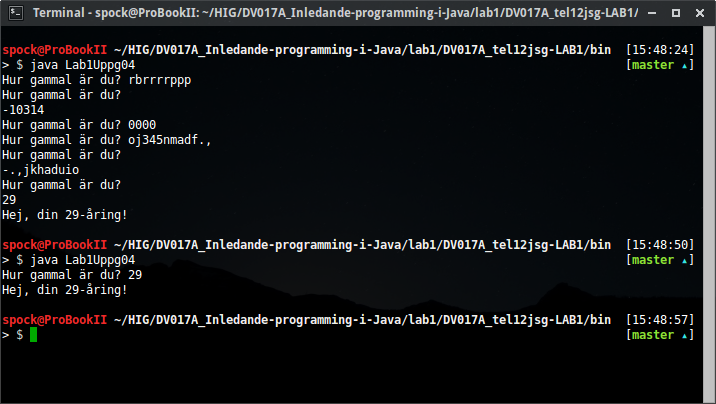
\includegraphics[width=\linewidth]{img/04.png}
    \caption{Körning av koden till Uppgift \ref{uppgift-4}}
    \label{fig:screenshot-04}
\end{figure}

    \section{Uppgift 5}\label{uppgift-5}

\subsection{Beskrivning}
\subsubsection*{Instruktioner}
\begin{verbatim}
5. Skriv ett program där användaren ska skriva in ett heltal. Programmet ska
   sedan skriva ut alla heltal från detta tal ner till ett. Du ska använda dig
   av en while-loop. Exempel på utskrift, användarens inmatning är markerat med
   fetstil/understrykning:

    Ange det heltal som du vill räkna ner från: *6*
    6 5 4 3 2 1
\end{verbatim}

\subsection{Kommentar}
% TODO: Kommentar på #5.

\subsection{Källkod}\label{uppgift-5_src}
\subsubsection*{Lab1Uppg05.java}
\inputminted[]{java}{src/Lab1Uppg05.java}

    \section{Uppgift 6}\label{uppgift-6}

\subsection{Instruktioner}
\begin{verbatim}
6. Skriv två program som ger samma utskrift som den i uppgift 5, men använd
   istället en for- loop i ena programmet och en do-loop i det andra.
\end{verbatim}

\subsection{Lösning}
\subsubsection{Funktion}
Programmet använder återigen samma logik för att kontrollera korrekt inmatning
men till skillnad från i Uppgift \ref{uppgift-4} och Uppgift \ref{uppgift-5}
används en funktion \texttt{getUserInput()}.
\par Koden blir modulär och enklare att hantera. Funktionens åtkomstmodifierare
\texttt{static} gör funktionen till en klassfunktion, alla objekt som
instanstieras från klassen delar funktionen. Funktionen hör till klassen, inte
objekten.
\texttt{protected} gör functionen ''synlig'' inom paketet.
\footnote{\url{https://docs.oracle.com/javase/tutorial/java/javaOO/classvars.html}}

\par Själva nedräkningen görs också inuti funktioner som anropas från
\texttt{main}.

\begin{description}
\item[\texttt{protected static void countDownUsingForLoop(int start)}] \hfill \\
räknar ner från parametervärdet \texttt{start} med hjälp av en \texttt{for}-loop

\item [\texttt{protected static void countDownUsingDoLoop(int start)}] \hfill \\
räknar ner från parameter värdet \texttt{start} med hjälp av en \texttt{do}-loop
\end{description}


\subsubsection{Kommentar}
\par I slutet av \texttt{main}-metoden avslutas programmet med
\texttt{System.exit(0);} där $0$ indikerar lyckad exekvering och allt annat än
noll nästan uteslutande är någon form av felkod, t.ex. $127$ för ''"command not found"''\ 
\footnote{\url{http://www.tldp.org/LDP/abs/html/exitcodes.html}}


\subsubsection{Källkod}\label{uppgift-6_src}
%\begin{listing}[H]
    \inputminted[linenos]{java}{src/Lab1Uppg06.java}
    \caption{Lab1Uppg06.java}
    \label{Uppg6src}
%\end{listing}

\subsubsection{Skärmdump}
\begin{figure}[htbp]
    \centering
        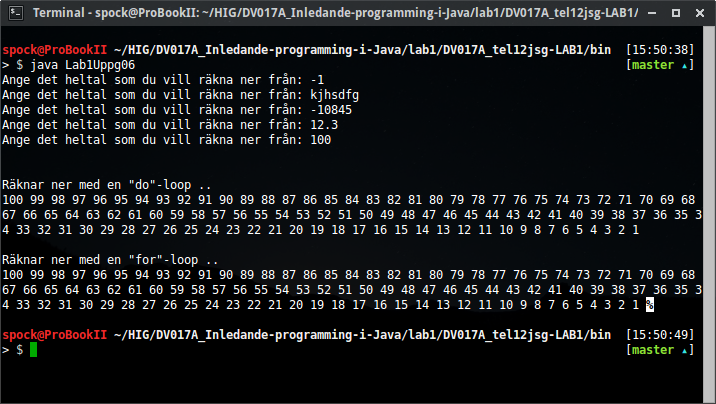
\includegraphics[width=\linewidth]{img/06.png}
    \caption{Körning av koden till Uppgift \ref{uppgift-6}}
    \label{fig:screenshot-06}
\end{figure}

    \section{Uppgift 7}\label{uppgift-7}

\subsection{Beskrivning}
\subsubsection*{Instruktioner}
\begin{verbatim}
7. Skriv ett program som låter användaren mata in värden till de tre
   heltalsvariablerna var1, var2 och var3. Programmet skall sedan för varje
   påstående a) – e) lagra värdet av påståendet i den booleska variabeln svar
   och därefter skriva ut värdet av svar , försett med lämplig ledtext:

    a) Talet var1 är jämnt delbart med 7.
    b) Talet var3 är inte jämnt delbart med talet var2.
    c) Talet var1 är större än minst något av talen var2 och var3.
    d) Talet var1 är större än talet var2, som i sin tur är större än talet var3.
    e) Talet var1 är större än ett av talen var2 och var3, men inte större än båda.

   Tips: För att kolla om något tal är jämnt delbart med ett annat,
         använd modulus-operatorn %!
\end{verbatim}

\subsection{Kommentar}
% TODO: Kommentar på %7.

\subsection{Källkod}\label{uppgift-7_src}
\subsubsection*{Lab1Uppg07.java}
%\begin{listing}[H]
    \inputminted[linenos]{java}{src/Lab1Uppg07.java}
    \caption{Lab1Uppg07.java}
    \label{Uppg7src}
%\end{listing}

    \section{Uppgift 8}\label{uppgift-8}

\subsection{Beskrivning}
TODO: Beskriving uppgift 8.

\subsection{Källkod}\label{uppgift-8_src}
%\subsubsection{Lab1Uppg08.java}
\inputminted[]{java}{../src/Lab1Uppg08.java}

    \section{Uppgift 9}\label{uppgift-9}

\subsection{Beskrivning}
TODO: Beskriving uppgift 9.

\subsection{Källkod}\label{uppgift-9_src}
%\subsubsection{Lab1Uppg09.java}
\inputminted[]{java}{../src/Lab1Uppg09.java}

    \section{Uppgift 10}\label{uppgift-10}

\subsection{Beskrivning}
TODO: Beskriving uppgift 10.

\subsection{Källkod}\label{uppgift-10_src}
%\subsubsection{Lab1Uppg010.java}
\inputminted[]{java}{../src/Lab1Uppg10.java}

%   \section{Resultat}\label{setup}
TODO: Eventuellt resultat och kommentar på hela labben.


    \newpage

    \section{Referenser}\label{referenser}

\subsection{www}\label{}
% ==============================================================================

\subsection{Literature}\label{}
% ==============================================================================

\subsection{Source files}\label{sources}
% ==============================================================================
Full source, including spice simulation files, CSV data, schematics, etc
TODO: is available at https://github.com/jonasjberg/FIX_URL


\end{document}
